\documentclass{article}
\usepackage{latexsym}
%\usepackage[utf8]{inputenx}
\usepackage[]{inputenx}
\usepackage[spanish]{babel}
\usepackage{graphicx}
\usepackage{anysize}
\usepackage{amsmath}
\usepackage{amssymb}
\usepackage{float}
\usepackage{fancyhdr}
\setlength{\skip\footins}{5cm}
\usepackage{lscape}
\usepackage{verbatim}
\usepackage{moreverb}
\usepackage{url}
\usepackage{listings}
\usepackage{enumitem}
\usepackage{multicol}
\usepackage{pifont}
\usepackage{listings}
\let\verbatiminput=\verbatimtabinput
\usepackage[nottoc,numbib]{tocbibind}
\setcounter{tocdepth}{3}
\setcounter{secnumdepth}{3}
\newcommand{\mayor}{\char60 }
\newcommand{\desc}{Capa Negocio- Recursos/Materiales - Grupo 2 - Tp Taller II - v 2.0 }
\newcommand{\menor}{\char62 }
\marginsize{2cm}{2cm}{.5cm}{3cm} 
\pagestyle{myheadings}
\renewcommand{\headrulewidth}{0.5pt}

\usepackage{sectsty}
\sectionfont{\LARGE}
\subsectionfont{\Large}
\subsubsectionfont{\large}
\paragraphfont{\large}
\usepackage{color}
\definecolor{gray}{rgb}{0.4,0.4,0.4}
\definecolor{darkblue}{rgb}{0.0,0.0,0.6}
\definecolor{cyan}{rgb}{0.0,0.6,0.6}
\definecolor{maroon}{rgb}{0.5,0,0}
\definecolor{darkgreen}{rgb}{0,0.5,0}
\lstset{
  basicstyle=\ttfamily\scriptsize,
  columns=fullflexible,
  showstringspaces=false,
  commentstyle=\color{gray}\upshape
}

\lstdefinelanguage{XML}
{
basicstyle=\ttfamily,
  morestring=[s]{"}{"},
  morecomment=[s]{?}{?},
  morecomment=[s]{!--}{--},
  commentstyle=\color{darkgreen},
  moredelim=[s][\color{black}]{>}{<},
  moredelim=[s][\color{red}]{\ }{=},
  stringstyle=\color{blue},
  identifierstyle=\color{darkblue}
}
\begin{document}

\lstset{language=XML,
        breaklines=true}
\begin{titlepage}

\newcommand{\HRule}{\rule{\linewidth}{0.5mm}} % Defines a new command for the horizontal lines, change thickness here

\center % Center everything on the page
 
%----------------------------------------------------------------------------------------
%	HEADING SECTIONS
%----------------------------------------------------------------------------------------

\textsc{\LARGE Universidad De Buenos Aires}\\[1.5cm] % Name of your university/college
\textsc{\Large Facultad De Ingeniería}\\[0.5cm] % Major heading such as course name
\textsc{\large 75.52 Taller de Programaci\'on II}\\[0.5cm] % Minor heading such as course title

%----------------------------------------------------------------------------------------
%	TITLE SECTION
%----------------------------------------------------------------------------------------

\HRule \\[0.4cm]
{ \huge \bfseries Recursos}\\ Capa de Negocios\\[0.4cm] % Title of your document
\HRule \\[1.5cm]
 
%----------------------------------------------------------------------------------------
%	AUTHOR SECTION
%----------------------------------------------------------------------------------------

% If you don't want a supervisor, uncomment the two lines below and remove the section above
\Large \emph{Integrantes:}\\

Hugo \textsc{Chavar} - 90541\\ % Your name
Dami\'an \textsc{Manoff} - 93169\\ % Your name
Yamila \textsc{Glinsek} - 93219\\ % Your name
Andr\'es \textsc{Sanabria} - 93403\\[5cm] % Your name

\textit{capanegocio.recursos@yahoo.com.ar}
%----------------------------------------------------------------------------------------
%	DATE SECTION
%----------------------------------------------------------------------------------------

{\large \text \em \today }\\[3cm] % Date, change the \today to a set date if you want to be precise
%{10 de Septiembre de 2013}
 
%----------------------------------------------------------------------------------------

\vfill % Fill the rest of the page with whitespace

\end{titlepage}
\tableofcontents
\newpage
\section{Introducci\'on}
Recursos da referencia a lo que podemos traducir como Archivos, Links y Encuestas.\\
Los servicios que brindamos son:
\begin{enumerate}
	\item Posibilitar la subida y descarga de archivos al sistema.
	\item Crear encuestas, que pueden ser o no \emph{Evaluadas}.
	\item Permitir el acceso a responder encuestas y realizar su evaluaci\'on seg\'un el criterio establecido por el creador de la misma.
	\item Linkear p\'aginas externas y/o internas de la web.
\end{enumerate}
\markboth{Capa Negocio}{\desc}	
\section{Definiciones}
\begin{description}
	\item Cosas que ya se han definido hasta el momento por la interacci\'on con los grupos y docentes:
	\renewcommand{\labelitemi}{\ding{85}} 
	\begin{itemize}
		\item Se utilizar\'a como IDE \emph{Eclipse} y plataforma \emph{Java 7}.
		\item La comunicaci\'on entre capas se realiza por Web Services.
		\item Los archivos van a ser pasados entre capas como multi-part (o similar) a trav\'es de dichos Web Services.
		\item Tanto con la capa de arriba (Presentaci\'on) como la de abajo (Integraci\'on) implementar\'an la interfaz en XML.
		\item Los archivos ser\'an pasados de nuestra capa a la  \emph{capa de Integraci\'on}  para que \'esta trate con el FileSystem o con la \emph{capa de Acceso a datos} como ha de ser almacenado. Queda por definirse si es necesario una conversaci\'on previa entre capas antes de la transferencia del archivo.
%\item 

	\end{itemize}
\end{description}

\section{Clases}
\subsection{Archivos}
	Para el manejo de archivos se tendr\'a la siguiente clase:
	
%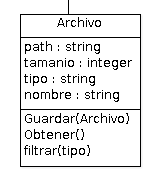
\includegraphics[scale=0.7]{Archivo.png}
\begin{figure}[h]
\centering
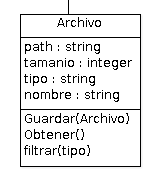
\includegraphics[scale=0.8]{Archivo}

\caption{Clase Archivo}
\end{figure}
	
\paragraph{\large{Atributos}}
	%La cual tiene como atributo:\
\begin{description}
		\item[path] que es una cadena que cuenta con la direccion en la cual se encuentra guardado en el file system el archivo.
		\begin{itemize}
			\item Tipo De Datos : String
			\item Longitud : 100
		\end{itemize}
		\item[tamanio] es el peso del archivo en Megabytes, por lo tanto es solo num\'erico. Consideraremos un maximo de 100 MB para cada archivo. Por lo tanto la longitud maxima del campo ser\'a 4 caracteres.
		\begin{itemize}
			\item Tipo De Datos : Integer
			\item Longitud : 10
		\end{itemize}
		\item[tipo] se refiere a la extensi\'on del Archivo (por ejemplo: mp3, mpeg4, doc).
		\begin{itemize}
			\item Tipo De Datos : String
			\item Longitud : 5
		\end{itemize}
		\item[nombre] es la identificaci\'on del archivo.
		\begin{itemize}
			\item Tipo De Datos : String
			\item Longitud : 40
		\end{itemize}
\end{description}

\subsection{Recurso}
\begin{figure}[H]
\centering
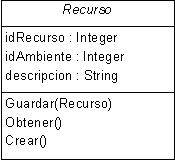
\includegraphics[scale=0.9]{recurso}
%\includegraphics[scale=0.45]{organ}\\ %, angle=90

\caption{Clase Recurso}
\end{figure}
\paragraph{\large{Atributos}}
\begin{description} 
\item[descripcion] Es el texto que ver\'a el usuario, sobre el cual puede hacer clic. \
\begin{itemize}
\item Tipo De Datos : String
\item Longitud : 100
\end{itemize}
\item[idAmbiente] Ambiente al cual pertenece el recurso.\
\begin{itemize}
\item Tipo De Datos : Integer
\item Longitud : 10
\end{itemize}
\item[idRecurso] Identificador del recurso.\
\begin{itemize}
\item Tipo De Datos : Integer
\item Longitud : 10
\end{itemize}
\end{description}
\subsection{Encuestas}
La idea de encuesta es algo del siguiente tipo:

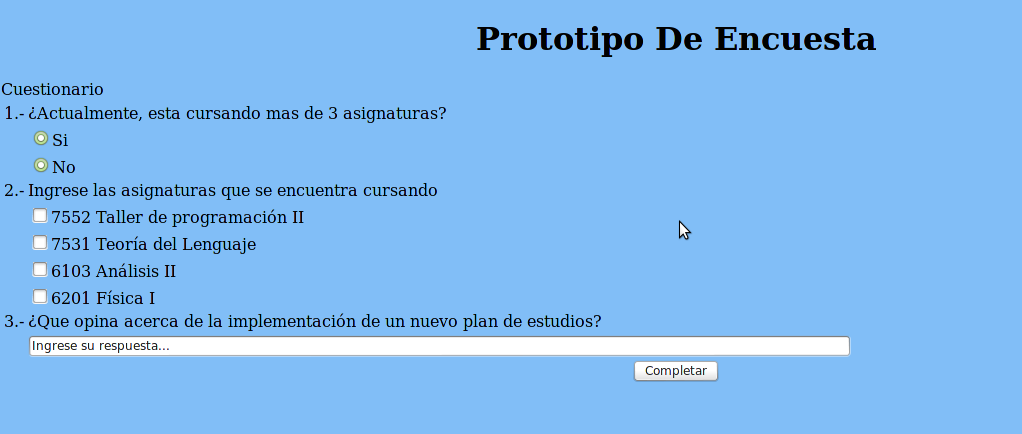
\includegraphics[scale=0.4]{EncuestaFoto.png}	

En donde claramente se pueden distinguir 3 tipos diferentes de preguntas:
\begin{enumerate}
\item Preguntas que solo admiten una opci\'on como respuesta.
\item Preguntas que admiten multiples opciones como respuesta.
\item Preguntas cuya respuesta es a completar.
\end{enumerate}

Adem\'as existir\'an dos tipos de encuestas:
\begin{enumerate}
\item Encuestas Evaluadas
\item Encuestas No Evaluadas.
\end{enumerate}

Con respecto al primer tipo de encuestas solo podremos admitir preguntas del tipo 1 y 2 ya que se dificulta la tarea de evaluar respuestas a completar.\\
Las encuestas del segundo tipo admitir\'an todo tipo de preguntas.

%Las encuestas se manejar\'an del siguiente modo:\\

%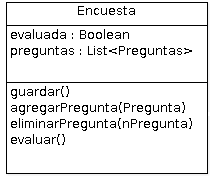
\includegraphics[scale=0.75]{Encuesta.png}

\begin{figure}[h]
\centering
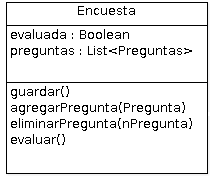
\includegraphics[scale=0.8]{Encuesta}

\caption{Clase Encuesta}
\end{figure}

%La cual se compone de los siguientes elementos:
\paragraph{\large{Atributos}}
\begin{description}
\item[evaluada] atributo de tipo booleano que se define en el constructor, es decir, \textit{new Encuesta(evaluada=true)}, por defecto las encuesta son no evaluadas.
\begin{itemize}
\item Tipo De Datos : Boolean
\item Longitud : 1
\end{itemize}
\item[preguntas] es una lista de preguntas. Como m\'aximo se aceptaran \textbf{30 preguntas por encuesta}. El id de cada pregunta estar\'a relacionado con la posici\'on que ocupen en la lista m\'as uno, es decir \textit{preguntas[0]} ser\'a la pregunta n\'umero 1 asociada a esa encuesta. 
\begin{itemize}
\item Tipo De Datos : List$<$Pregunta$>$
\item Longitud : 30
\end{itemize}
\end{description}

Dicho esto tendremos que definir las preguntas que tendremos. En nuestro caso habr\'a dos tipos de preguntas
\begin{enumerate}
\item Pregunta : Es la clase padre donde la respuesta esperada podria ser m\'ultiple o bien una descripci\'on.
\item PreguntaRespuestaFija : son aquellas preguntas en donde el que la crea define las respuestas posibles, y el que las responde tiene la posibilidad de elegir una o mas respuestas, seg\'un lo defina el creador.En el prototipo son las preguntas 1 y 2.
\end{enumerate}
%\textsc{Pregunta}\\
\subsection{Pregunta} \

%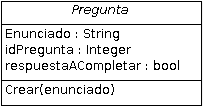
\includegraphics[scale=0.75]{Pregunta.png}

\begin{figure}[h]
\centering
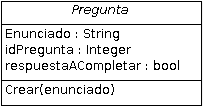
\includegraphics[scale=0.8]{Pregunta}

\caption{Clase Pregunta}
\end{figure}

\paragraph{\large{Atributos}}
\begin{description}


\item[enunciado] ser\'a la pregunta en s\'i.
\begin{itemize}
\item Tipo De Datos : String
\item Longitud : 200
\end{itemize}
\item[idPregunta]  el id de la pregunta corresponde a un entero que identifique cada pregunta dentro de una encuesta
\begin{itemize}
\item Tipo De Datos : Integer
\item Longitud : 2
\end{itemize}
\item[respuestaACompletar] es un booleano que muestra si una respuesta es a completar o es de opcion m\'ultiple. Por defecto todas las preguntas son a completar. En caso contrario se deber\'a crear una \textit{PreguntaRespuestaFija}
\begin{itemize}
\item Tipo De Datos : Boolean
\item Longitud : 1
\end{itemize}
\end{description}
%\textsc{PreguntaRespuestaFija}:\\
\subsection{PreguntaRespuestaFija} \

%Estas preguntas tendr\'an el siguiente formato:\\

%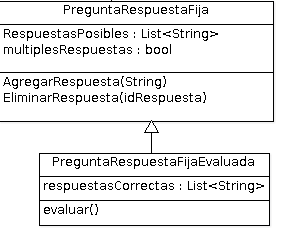
\includegraphics[scale=0.75]{RespuestaFija.png}

\begin{figure}[h]
\centering
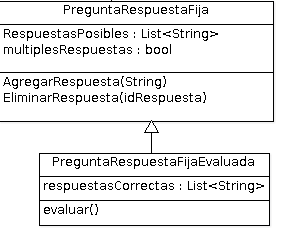
\includegraphics[scale=0.9]{RespuestaFija}

\caption{Clase PreguntaRespuestaFija}
\end{figure}

\paragraph{\large{Atributos}}

\begin{description}

\item[m\'ultiplesRespuestas] define si la pregunta aceptar\'a mas de una respuesta. Por defecto las m\'ultiples respuestas est\'an desabilitadas.
\begin{itemize}
\item Tipo De Datos : Boolean
\item Longitud : 1
\end{itemize}
\item[respuestasPosibles] es una lista de tamaño m\'aximo 6, es decir una pregunta a lo sumo podr\'a tener 6 respuestas correctas. Las respuestas se distinguen seg\'un la posici\'on que ocupan dentro de la lista, es decir si respuestaPosible[0] = Fiuba , la respuesta fiuba estar\'a asociada a la primera posici\'on de la lista.\\
Vale aclarar que si las multiples respuestas est\'an apagadas, la lista contendr\'a si y solo si una respuesta, y no permitir\'a agregar m\'as.\\
\begin{itemize}
\item Tipo De Datos : List $<$String$>$
\item Longitud : 6
\end{itemize} 
\item A la vez, como este tipo de preguntas es posible evaluar habr\'a una clase \textbf{PreguntaRespuestaFijaEvaluada} la cual tendr\'a las opciones correctas que se esperan.\\

\begin{itemize}
	\item RespuestasCorrectas : esta lista contendr\'a los/el id de las respuestas que se consideran correctas. Es decir el tamaño ser\'a desde 0 a la cantidad de Respuestas agregadas en la instancia anterior. Como valor m\'aximo se especificar\'a el valor 6 en el caso de que todas las respuestas sean correctas.
	\begin{itemize}
\item Tipo De Datos : List$<$Integer$>$
\item Longitud : 6
\end{itemize} 
\end{itemize}

\end{description}

% andy
\subsection{Encuesta Respondida} 

%Estas preguntas tendr\'an el siguiente formato:\\

%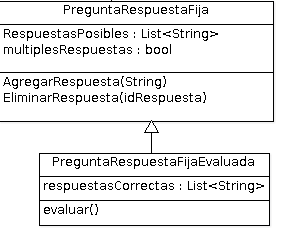
\includegraphics[scale=0.75]{RespuestaFija.png}

\begin{figure}[h]
\centering
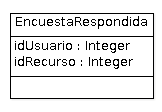
\includegraphics[scale=0.9]{EncuestaRespondida}

\caption{Clase EncuestaRespondida}
\end{figure}

\paragraph{\large{Atributos}}

\begin{description}
\item[idUsuario] permite relacionar la encuesta respondida con el usuario que se encargo de completarla.
\begin{itemize}
\item Tipo De Datos : Integer
\item Longitud : 20
\end{itemize}

\item[idRecurso] Identificador del recurso perteneciente a la encuesta que responde la EncuestaRespondida.
\begin{itemize}
\item Tipo De Datos : Integer
\item Longitud : 10
\end{itemize} 
\end{description}

\subsection{Pregunta Respondida} 

\begin{figure}[h]
\centering
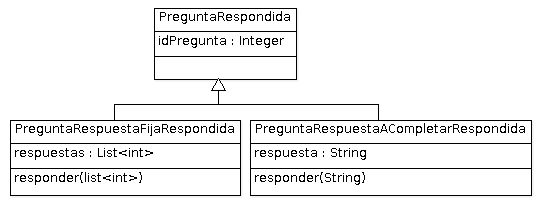
\includegraphics[scale=0.9]{PreguntaRespondida}

\caption{Clase PreguntaRespondida}
\end{figure}

\paragraph{\large{Atributos}}

\begin{description}
\item[idPregunta] identificador de la pregunta dentro de la encuesta.
\begin{itemize}
\item Tipo De Datos : Integer
\item Longitud : 10
\end{itemize} 
\item A su vez, las preguntas respondidas podr\'an ser fijas o a completar, siendo la forma de responderlas en ambos casos distintas. 
\end{description}

\subsubsection{Respuesta Fija Respondida}

\begin{description}
\item[respuestas] por tratarse de posibles respuestas a las preguntas de respuesta fija de una Encuesta, este atributo es tambi\'en una lista de tamaño m\'aximo 6, es decir, se podr\'a responder como m\'aximo 6 respuestas. Las respuestas se distinguen seg\'un la posici\'on que ocupan dentro de la lista de la Encuesta original.
\begin{itemize}
\item Tipo De Datos : List $<$Integer$>$
\item Longitud : 6
\end{itemize}
\end{description}

\subsubsection{Pregunta Respuesta a Completar Respondida}

\begin{description}
\item[respuesta] Atributo que guarda la respuesta proporcionada por el usuario respondente. Al ser una respuesta a completar, se admite un \'unico texto.
\begin{itemize}
\item Tipo De Datos : String
\item Longitud : 100
\end{itemize} 
\end{description}
% andy



\subsection{Links}

Los links ser\'an las referencias a otros sitios webs o referencias a articulos dentro de este mismo sitio.

\begin{figure}[h]
\centering
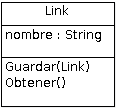
\includegraphics[scale=0.9]{Links}

\caption{Clase Link}
\end{figure}

%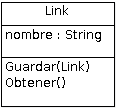
\includegraphics[scale=0.75]{Links.png}

\paragraph{\large{Atributos}}
\begin{description}
\item[nombre] es el path adonde apunta el hiperv\'inculo.% Definiremos como tamaño m\'aximo 200 carateres.
\begin{itemize}
	\item Tipo De Datos : String
	\item Longitud : 200
\end{itemize}
\end{description}


\markboth{Capa Negocio}{\desc}	
\section{Diagrama de Clases}
	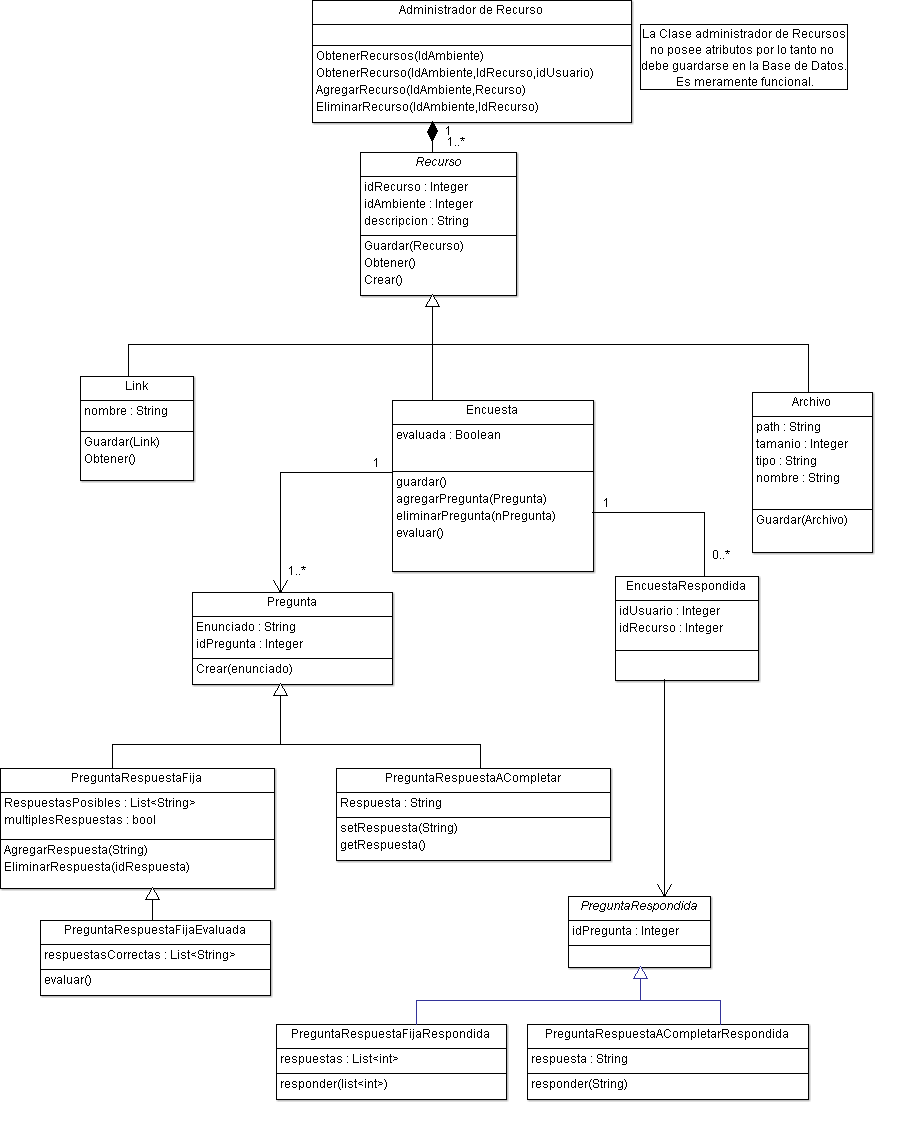
\includegraphics[scale=0.55]{Diagramadeclase6.png}
\markboth{Capa Negocio}{\desc}	
\pagebreak
	

\section{Interfaces}
	\begin{description}
		\item[Provistas a la capa de Presentaci\'on ] \
		\renewcommand{\labelitemi}{\ding{105}} 
		\begin{itemize}
		\item \emph{OBTENER RECURSO}:
			Este m\'etodo devuelve ya sea un Archivo, un Link o una Encuesta segun lo que se solicite. Es requisito tener el ID de recurso a consultar por lo que primero deben obtenerse con \emph{OBTENER LISTA RECURSOS}.
			\begin{description}
				\item[INPUT] XML\_PARAMETROS
				\item[OUTPUT] XML\_RESULTADO\\
			\end{description}
		

			Como par\'ametro se necesitan los siguientes items detallados de la siguiente forma:
				
\begin{lstlisting}
<parametro>
  <recurso>
    <recursoId>INT idDelRecurso</recursoId>
    <tipo>STRING tipo (ARCHIVO,LINK,ENCUESTA)</tipo>
  </recurso>
</parametro>
\end{lstlisting}
				
			Como resultado se obtendr\'an los siguientes archivos dependiendo la respuesta del servicio:
			

		\begin{itemize}
			\item ARCHIVO 
			
			\lstinputlisting{archivo.xml}	
			\textbf{Donde el tag \emph{rawFile} contiene un archivo serializado con JAXB, el tipo de dato que devuelve es un DataHandler, el cliente para deserializar debe poseer una clase con el siguiente atributo:} \newline
			\begin{verbatim}
				@XmlElement(name = "rawFile")
				@XmlMimeType("application/octet-stream")
				private DataHandler dataHandler;
			\end{verbatim}
			
			\item LINK
			
			\lstinputlisting{link.xml}
\clearpage
			
			\item ENCUESTA NO EVALUABLE
			
			\lstinputlisting{encuestaNoEvaluada.xml}
			
			\item ENCUESTA EVALUABLE
									
			\lstinputlisting{encuestaEvaluada.xml}
\textbf{Notar que existen dos tags para las preguntas \emph{preguntaConOpciones} y \emph{preguntaSinOpciones} para diferenciar las que deben ser completadas en un TextBox de las que usan un mecanismo para tildar la/s opcion/es correcta/s. Dentro de \emph{preguntaConOpciones} se diferencian por el atributo \textit{multiplesCorrectas}, para que sea posible elegir una o muchas, esto hay que hacerlo debido a que una pregunta puede ser marcada como \textit{multiplesCorrectas = "true"} pero tenga una sola que es correcta.\newline
Se enviar\'a \textit{multiplesCorrectas = "false"} cuando no hayan respuestas correctas, es decir, cuando no sea evaluable la encuesta.  } \newline

\textbf{Adem\'as, tener en cuenta que las respuestas en las preguntasConOpciones arrancan en 1, y no en 0 como se hab\'ia definido inicialmente, quedando sus posibles valores definidos entre 1 y la cantidad de respuestasPosibles.  } \newline
		
		\end{itemize}
%\clearpage
			\item Los posibles errores detectados se mostrar\'an de la siguiente manera:
			\begin{itemize}
				\item ERROR PARAMETROS INVALIDOS EN GENERAL
				
				\lstinputlisting{parInvalidos.xml}
				
				\item ERROR PARAMETROS ESPEC\'IFICOS INVALIDOS FALTA EL TIPO
				
				\lstinputlisting{materialInvalido.xml}		
								
				\item ERROR PARAMETROS ESPEC\'IFICOS INVALIDOS FALTA EL ID RECURSO:
				
				\lstinputlisting{idRecursoInvalido.xml}	
				
				\item ERROR PARAMETROS ESPEC\'IFICOS INVALIDOS TIPO DE RECURSO INEXISTENTE (los v\'alidos son: Link, Encuesta y Archivo):
				
				\lstinputlisting{recursoInvalido.xml}				
				
				\item ERROR AL OBTENER RECURSO:
				
				\lstinputlisting{recursoNoAlcanzable.xml}
				
				\item CAPA DE INTEGRACION INDICA QUE NO HAY DATOS:
				
				\lstinputlisting{respuestaVacia.xml}
				
				\item ERRORES PROVENIENTES DE LA CAPA DE INTEGRACION:
				
				\lstinputlisting{errorIntegracion.xml}
				
			\end{itemize}
			\clearpage
			\item \emph{OBTENER LISTA RECURSOS}
			\begin{description}
				\item[INPUT] ID-AMBIENTE
				\item[OUTPUT] LISTA-DE [ID-RECURSO, DESCRIPCION, TIPO]\\
			\end{description}
			\lstinputlisting{recursos.xml}
	
			\item \emph{AGREGAR ARCHIVO}
		%	\begin{description}
				Este WS recibe un xml con la MetaData del archivo, y un byte array que contiene al archivo a agregar:
				El xml debe cumplir la siguiente especificaci\'on:
				
		%	\end{description}
			\lstinputlisting{Agregar/archivo.xml}	
			
			\item \emph{AGREGAR RECURSO} Aclaraci\'on: este WS no es compatible con la parte de archivos. VER AGREGAR ARCHIVO.
			\begin{description}
				La utilidad es la adicción de LINKS y ENCUESTAS.
				Para ello recibe los siguientes parametros:
				 LINKS:
				 
				 \lstinputlisting{Agregar/link.xml}	
				 
				 ENCUESTA:
				 
				 \lstinputlisting{Agregar/encuesta.xml}	
			\end{description}
%			\item \emph{AGREGAR ENCUESTA}
%			\begin{description}
%				\item[INPUT] ID-AMBIENTE, DESCRIPCI\'ON, ENCUESTA 
%				\item[OUTPUT] MENSAJE DE CONFIRMACI\'ON\\
%			\end{description}
%			\item \emph{GUARDAR ENCUESTA RESPONDIDA}:  Es requisito tener el ID de recurso a consultar por lo que primero deben obtenerse con \emph{OBTENER LISTA RECURSOS}.
%			\begin{description}
%				\item[INPUT] ID-ENCUESTA, ID-USUARIO, LISTA-RESPUESTAS
%				\item[OUTPUT] MENSAJE DE CONFIRMACI\'ON \\
%			\end{description}
%			\item \emph{OBTENER ENCUESTA RESPONDIDA}:  Es requisito tener el ID de recurso a consultar por lo que primero deben obtenerse con \emph{OBTENER LISTA RECURSOS}.
%			\begin{description}
%				\item[INPUT] XML\_PARAMETROS
%				\item[OUTPUT] XML\_RESULTADO\\
%			\end{description}
			
Como par\'ametro se necesitan los siguientes items detallados de la siguiente forma:
				
\begin{lstlisting}
<parametro>
  <recurso>
    <recursoId>INT idDelRecurso</recursoId>
  </recurso>
  <usuarioId>INT idDelUsuario</usuarioId>
</parametro>
\end{lstlisting}	

De ser exitoso la ejecuci\'on se obtendr\'an las siguientes respuestas del servicio:		

		\begin{itemize}
			\item ENCUESTA RESPONDIDA EVALUADA
			
			\lstinputlisting{encuestaRespondidaEvaluada.xml}
			
			\item ENCUESTA RESPONDIDA NO EVALUADA
			
			\lstinputlisting{encuestaRespondidaNoEvaluada.xml}
		\end{itemize}
		
		\textbf{Tener en cuenta que las respuestas en las preguntasRespondidasConOpciones arrancan en 1, y no en 0 como se hab\'ia definido inicialmente, quedando sus posibles valores definidos entre 1 y la cantidad de respuestasPosibles.  } \newline
			\item \emph{BORRAR RECURSO}:  Es requisito tener el ID de recurso a consultar por lo que primero deben obtenerse con \emph{OBTENER LISTA RECURSOS}.
			\begin{description}
				\item[INPUT] ID-AMBIENTE, ID-RECURSO
				\item[OUTPUT] MENSAJE DE CONFIRMACI\'ON \\
			\end{description}
		
				
		\end{itemize}
%		\renewcommand{\labelitemi}{\ding{118}} 
%		\item[Requeridas a la capa de Integraci\'on \emph{( incompleto)}] \
%		\\Nota:
%		\emph{ En un principio, no necesitaremos que la capa de integraci\'on haga joins de tablas de Base de Datos, ya que todo va a ser requerido por ID.}
%		\begin{itemize}
%			\item \emph{OBTENER LISTA RECURSOS}
%			\begin{description}
%				\item[INPUT] ID-AMBIENTE
%				\item[OUTPUT] LISTA-DE [ID-RECURSO, DESCRIPCION, TIPO]
%			\end{description}
%			\item \emph{OBTENER RECURSO}
%			\begin{description}
%				\item[INPUT] ID-AMBIENTE, ID-RECURSO
%				\item[OUTPUT] LINK-AL-RECURSO
%			\end{description}
%			\item \emph{OBTENER ARCHIVO}
%			\begin{description}
%				\item[INPUT] LINK-AL-ARCHIVO
%				\item[OUTPUT] ARCHIVO
%			\end{description}
%			\item \emph{AGREGAR RECURSO}
%			\begin{description}
%				\item[INPUT] ID-AMBIENTE, DESCRIPCI\'ON, TIPO, DATOS (\emph{Difiere seg\'un tipo de recurso})
%				\item[OUTPUT] MENSAJE DE CONFIRMACI\'ON \'o LINK-AL-RECURSO
%			\end{description}
%			\item \emph{BORRAR RECURSO}
%			\begin{description}
%				\item[INPUT] ID-AMBIENTE, ID-RECURSO
%				\item[OUTPUT] MENSAJE DE CONFIRMACI\'ON
%			\end{description}
%		\end{itemize}
	\end{description}
	\markboth{Capa Negocio}{\desc}
\end{document}
